
\documentclass[conference]{IEEEtran}
\IEEEoverridecommandlockouts

\usepackage{cite}
\usepackage{amsmath,amssymb,amsfonts}
\usepackage{algorithmic}
\usepackage{algorithm}
\usepackage{graphicx}
\usepackage{textcomp}
\usepackage{xcolor}
\usepackage{booktabs}
\usepackage{hyperref}
\usepackage{array}

\graphicspath{{images/}}

\def\BibTeX{{\rm B\kern-.05em{\sc i\kern-.025em b}\kern-.08em
    T\kern-.1667em\lower.7ex\hbox{E}\kern-.125emX}}

\begin{document}

\title{Resilient WMN Routing via Digital Twin-Augmented Graph Attention Reinforcement Learning}

\author{
  \IEEEauthorblockN{\small Anandakrishnan K V}
  \IEEEauthorblockA{\footnotesize
    \textit{Department of}\\
    \textit{Computer Science and IT,}\\
    \textit{School of Computing,}\\
    \textit{Amrita Vishwa Vidyapeetham, Kochi, India}\\
    anandakrishnankv23@gmail.com
  }
  \and
  \IEEEauthorblockN{\small Sreelekshmi S}
  \IEEEauthorblockA{\footnotesize
    \textit{Department of}\\
    \textit{Computer Science and IT,}\\
    \textit{School of Computing,}\\
    \textit{Amrita Vishwa Vidyapeetham, Kochi, India}\\
    sreelekshmis@kh.amrita.edu
  }
  \and
  \IEEEauthorblockN{\small Drupad M D}
  \IEEEauthorblockA{\footnotesize
    \textit{Department of}\\
    \textit{Computer Science and IT,}\\
    \textit{School of Computing,}\\
    \textit{Amrita Vishwa Vidyapeetham, Kochi, India}\\
    drupadmdas@gmail.com
  }
}

\maketitle

\begin{abstract}
Wireless Mesh Networks (WMNs) rely on dynamic connectivity between nodes, which helps in making it a flexible network architecture. This dynamicity can in turn result in these networks being susceptible to interferences. These interferences may be of malicious intent such as jamming attacks. Attacks or environmental interferences can degrade the transmission of data and affect the routing pathways. Since the conventional routing protocols do not handle these kinds of situations without any modifications, this paper introduces a method to overcome these challenges by inherent design. By using Digital Twin to simulate network behaviours and a Graph Attention Network (GAT) to extract the features of the network traffic and topology, the system can generate information enriched state embeddings. These embeddings can be used by a multi-agent Deep Q-Network (DQN) to make informed routing decisions.
\end{abstract}

\begin{IEEEkeywords}
Digital twin, resilient routing, jamming detection, Deep Q-Network, GAT.
\end{IEEEkeywords}

%------------------------------------------------------------------
\section{Introduction}

Wireless communications have been a practical solution in many use cases when compared to physical transmission mediums, however, the restricted range becomes a huge obstacle to cross. Wireless Mesh Networks (WMNs) helps to overcome this issue by using multi-hop routing. This helps to extend the range of data transmission through intermediary nodes. This decentralization makes it a viable option in many use cases like IoT, industrial automation and disaster response. Unfortunately, this flexibility is susceptible to vulnerabilities. Malicious attacks can target these networks to cut off inter-node connections, affect reliability, delay the transmission, and affect the overall effectiveness of the network.

Being resilient against these problems is challenging using the conventional mechanisms. Conventional methods include rule-based routing and heuristic topology control. They lack the adaptability required for dynamic environments. Moreover, mathematical optimization models, which are used for dynamic scenarios, tends to be quite heavy on resources when it comes to large networks. This is where Reinforcement Learning (RL) helps to find a balance between adaptability and being less computationally expensive in the execution time. There is, however, one drawback RL based routings face in WMNs, which is the centralization of the training. This goes against the fundamental principle of Mesh Networks.

As an answer to these challenges, we present our approach that unifies Digital Twin modelling, Graph Attention Networks, and Multi-Agent Deep Q-Networks. This integration provides the base for effective detection and fault tolerance of interferences in resilient WMNs.

Now to understand the proposed architecture, let us understand the core technologies:

\textbf{Digital Twin (DT):} It functions as a real-time virtual mirror of the physical infrastructure. The DT is also a testing ground for predictive analysis and anomaly detection. It actively monitors for differences between expected and actual radio signals. This would help in detecting jamming attacks.

\textbf{Multi-Agent Deep Q-Network (MADQN):} This extends traditional reinforcement learning by enabling collaborative adaptation across the network. Embedded agents within each node optimize local routing performance using individual policy networks applied over a global graph embedding. Together, these agents share training experiences via a common replay pool to improve global network efficiency.

\textbf{Graph Attention Network (GAT):} It is a type of Graph Neural Network (GNN) that uses attention mechanisms like transformers. It extracts vital structural features from the WMN. It aggregates neighbor-node information using learned attention weights to produce node embeddings. These embeddings help the MADQN to make routing decisions and assist in identifying topological anomalies.

These elements together will form the foundation of a dynamic routing solution that can detect threats as well as adapt to ever-changing network conditions. The importance of such resilient systems is evident in recent WMN research. In recent research, heuristic protocols have been largely neglected in favour of machine learning models. This change is required to manage the complexity that comes with modern networks.

%------------------------------------------------------------------
\section{Related Works}

Recent advancements in Wireless Mesh Networks shows a shift from rule-based and rigid protocols to dynamic solutions that implement machine learning. This is directly influenced by challenges faced in modern networking scenarios where there are needs of node mobility, increased interferences, and unpredictable traffic patterns.

\subsection{GNNs and Reinforcement Learning in Routing}

\textbf{Deep Reinforcement Learning (DRLR) and GNNs:} One of the main challenges in traditional RL is the incapacity to handle new changes in network topology without retraining. Pappone et al. (2023) fixed this by joining GNNs with Multi-Agent DRL. By using GNNs to understand the structure of the network state and store them as embeddings. The agents can then use these information-rich embeddings to make adaptive decisions across unfamiliar graphs.

For disaster response environments, Jin et al. (2025) introduced the Deep Reinforcement Learning-based Resilient Routing (DRLRR) approach. Since the standard Q-learning is prone to overestimation bias, their proposed model utilized Double Deep Q-Networks (DDQN). This ensures communication stability by tracking topology changes, optimizing the messaging formats and using the node-link data into a reward function.

\textbf{Graph Convolutional Networks (GCN):} gained popularity in 2017 thanks to Kipf and Welling. The objective was for the model to learn on graphs using an efficient spectral approximation of convolution. According to this approach, each node's representation is repeatedly refined by including the features of its local neighbors, which are then normalized by the degrees of the related nodes. During convolution, the convolutional GCN assumes a constant graph structure and uses only the adjacency of the graph (i.e., structural connectivity) to determine aggregation of weights instead of learned pairwise significance scores. With this architecture, information on graphs can be encoded in a computationally efficient manner. Formally, a GCN's layer-wise propagation rule is as follows:

\begin{equation}
H^{(l+1)} = \sigma\left(\tilde{D}^{-\frac{1}{2}}\tilde{A}\tilde{D}^{-\frac{1}{2}}H^{(l)}W^{(l)}\right)
\end{equation}

\noindent Where:
\begin{itemize}
    \item $\tilde{A} = A + I_N$ is the adjacency matrix with added self-connections.
    \item $\tilde{D}$ is the degree matrix of $\tilde{A}$.
    \item $W^{(l)}$ is the layer-specific trainable weight matrix.
    \item $\sigma$ is a non-linear activation function (e.g., SELU).
\end{itemize}

\textbf{Graph Attention Network (GAT):} In 2018 Veli\v{c}kovi\'{c} et al. developed GAT which introduces a more detailed architecture that is essential for robust routing. In contrast to GraphSAGE, which gives all neighbours simple equal or fixed weights, GATs obtain attention coefficients $\alpha_{ij}$ by using a self-attention mechanism. $\alpha_{ij}$ shows how important neighbor $j$ is to node $i$.

\begin{equation}
\alpha_{ij} = \frac{\exp\left(\text{LeakyReLU}\left(\vec{a}^T\left[W\vec{h_i} \| W\vec{h_j}\right]\right)\right)}{\sum_{k \in \mathcal{N}_i} \exp\left(\text{LeakyReLU}\left(\vec{a}^T\left[W\vec{h_i} \| W\vec{h_k}\right]\right)\right)}
\label{eq:gat}
\end{equation}

In practice, the GAT architecture handles many of the dynamic features of WMNs more effectively than GCN. Unlike GCN, which assigns uniform weights during aggregation, GAT selectively weights each neighbour's contribution through a learnable attention mechanism. This makes it suitable for environments where link reliability varies due to jamming or interference. This selective aggregation allows GAT to better capture the importance of high-quality, non-jammed links during routing, which is the core motivation behind its adoption in this framework.

\subsection{Fault and Anomaly Detection}

Understanding the current condition of the network directly impacts the routing performance. It is important to determine whether a disruption is the consequence of a routine malfunction or something more intentional before making any routing decisions.

\textbf{Digital Twin for Radio Environments:} What Krause et al. (2023) introduced was a rethinking of how anomaly detection works in radio environments. Instead of anchoring detection to patterns mined from past data, their system keeps a physics-based virtual replica of the network running alongside it in real time. A ray-tracing engine inside that replica works out what RSSI readings across each link ought to look like under normal conditions. Those calculated values become references. Any meaningful gap between predicted and measured signals gets flagged thereby avoiding any attack examples needed for training. Crucially, the framework can tell jamming apart from ordinary fading, which is exactly where conventional statistical detection tends to fall apart.

\subsection{Gap Analysis}

Pappone et al. (2023) built a solid routing foundation, yet the work overlooks the subtleties of physical layer threats by anchoring itself to standard network metrics. Krause et al. (2023) take a different angle leveraging digital twins for detection but deliberately stop at observation, leaving the door closed on any form of active network intervention.

Existing work has yet to meaningfully explore the integration of these two systems, mainly the idea of feeding high-fidelity anomaly scores from a Digital Twin directly into a Graph Attention Network (GAT) as live, dynamic features. This paper takes a step into that gap. The core proposition is that routing the Digital Twin's ground-truth awareness through the attention mechanism of a GAT-based reinforcement learning agent enables the network to build genuine resilience, where interference is anticipated and routed around before packet loss has a chance to escalate.

%------------------------------------------------------------------
\section{Proposed Framework}

This section will explore this routing framework in more detail. It will integrate a Digital Twin-based network model and a Graph-based Reinforcement Learning approach to improve the routing process. The outcome will be a system that is not only complex in its decision-making, but also agile in its responses.

\subsection{Digital Twin}

This framework is based on the Digital Twin (DT) concept, which is accomplished through the use of a specific Mesh Digital Twin module. Moreover, unlike traditional routing schemes, which are based on packet-based feedback, the Digital Twin concept takes a step further by utilizing a virtual representation of the real network, which is updated according to the current state of the network.

Digital Twin includes the following parts:

\textbf{Radio Map:} This is done through the collection of environmental radio maps that include Received Signal Strength (RSS) data, which is directly related to link-level performance characteristics such as latency and bandwidth capacity. These values are interpreted using sigmoidal transformation functions, which convert the RSS values into usable estimations. This is done in order for the Digital Twin to be able to factor in non-linear signal propagation characteristics that might otherwise be missed. It also factors in real-time changes in channel conditions as well as the presence of interfering signals.

\textbf{Feature Enrichment and Anomaly Awareness:} In order to enhance the awareness of the environment, the Digital Twin uses special modules named AnomalyBridge and JammerDetector. These modules enhance the quality of the network graph by adding more features to the nodes. In the nodes, the features are represented by a seven-dimensional vector. The features are the source indication, the destination indicator, the average latency, the average bandwidth, the anomaly score, the likelihood of jamming, and the neighbor's average jamming.

These features give the agent an improved sense of the status of the network and the difficulties it may face in the environment. It also allows the agent to deal with disruptions it has not experienced before.

\subsection{Graph Attention Networks}

The proposed framework uses a Graph Attention Network (GAT) to make decisions. The main aim of GAT is to learn the network structure and the interconnectedness of individual nodes.

% FIX 1: Removed stray text "Yes, the contents are the same. Here is the LaTeX:" from document body

\textbf{Input Representation:} The input representation of GAT is the seven-dimensional feature vector described earlier. The graph-based nature of GAT enables it to learn both from the topological information and the environmental information present in the network.

\textbf{Message Passing:} Information is transmitted between neighboring nodes via two Graph Attention Network layers. The attention mechanism enables each node to selectively focus on adjacent neighbours who are most important to the routing process. This allows vital information about node failures or jamming assaults to spread throughout the network, directly altering the representations of surrounding nodes. The SELU activation function is used between the GAT layers to keep self-normalizing features intact during message transfer.

\textbf{Q-Value Estimation:} The output embeddings generated by the attention layers are fed via fully connected layers to compute the Q-values. Each Q-value represents the estimated benefit that the agent will receive by selecting a specific neighbour as the next hop. Routing decisions are regarded as distinct actions, with each action resulting in a reward that drives the agent's decision-making process.

\subsection{Deep Q-Network Learning}

The learning mechanism is inspired by the Deep Q-Network architecture, which has been developed to work in a graph-like environment such as a mesh network. To make informed decisions, the agent uses the state representation provided by the GAT and combines it with Reinforcement Learning. The key aspects of the learning mechanism are:

\textbf{Experience Replay:} During training, interaction tuples $(s, a, r, s')$ are collected and stored in a replay memory. Random subsets are then drawn from this memory to form training batches. This random sampling breaks the temporal correlations that would otherwise exist between consecutive training samples, leading to improved convergence stability throughout the learning process.

\textbf{Exploration Strategy:} The framework uses an epsilon-greedy approach to find a balance between investigating new possibilities and capitalizing on what has previously been learned. During the initial rounds of training, the agent is encouraged to freely explore the surroundings. As training advances, the exploration rate $\varepsilon$ steadily decays, causing the agent to depend more heavily on its learnt rules.

\subsection{Reward Function}

Incentives are offered based on the routing decisions made by the agent. The incentives are designed to motivate the agent for efficient routing and also discourage futile efforts in routing.

\textbf{Base Reward:} The base reward is decided by the agent's movement towards the target. This promotes a less-hop, more-reward approach, where shorter pathways give higher rewards.

\textbf{Anomaly Penalization:} When an agent sends traffic through unstable nodes, a penalty is imposed. The overall reward is modified using an anomaly dampening factor:

\begin{equation}
R = R_{\text{base}} \times (1 - \alpha \times \text{AnomalyScore}) - \lambda_{\text{jam}} \times \mathbb{1}[\text{jammed}] + R_{\text{resilience}}
\end{equation}

\noindent Where $\alpha = 0.3$ denotes the anomaly dampening factor, $\lambda_{\text{jam}} = 0.5$ represents the jamming penalty coefficient, $\mathbb{1}[\text{jammed}]$ is an indicator function that takes the value 1 whenever the agent passes through a jammed node, and $R_{\text{resilience}} = 0.3$ is a bonus reward granted exclusively when the packet successfully reaches the destination without passing through any jammed node.

\textbf{Jamming Penalty:} A negative reward is given if the agent selects a node that is identified as jammed. This will deter the agent from passing through areas of the network where a great deal of interference is taking place.

\textbf{Resilience Incentive:} A new reward is provided when the routing process is finished successfully. This underlines the significance of the successful completion of the routing process, thereby adding to the overall resilience of the network.

\begin{figure}[htbp]
  \centering
  \includegraphics[width=\linewidth]{algorithm.png}
  %\caption{Resilient Routing Algorithm: MA GAT+DT training procedure.} % FIX 2: Added missing \caption
  \label{fig:algorithm} % FIX 3: Added missing \label
\end{figure}

%------------------------------------------------------------------
\section{Experiments and Results}

\subsection{Experimental Setup}
To assess the performance of the proposed MA GAT+DT routing protocol, a head-to-head comparison was carried out between the MA GAT+DT and a GAT-based routing baseline on a 50-node wireless mesh network across 3,000 training episodes. Two models were put to the test:
\begin{enumerate}
    \item \textbf{GAT Baseline (4 Features):} A single-agent GAT model that draws upon basic node properties, such as network connectivity and spatial location, while leaving out cooperative agent behaviour and dynamic environmental conditions.
    \item \textbf{MA GAT+DT (7 Features):} The proposed model enriches the baseline feature set with three additional DT-derived parameters: anomaly score, jamming probability, and neighbour jamming average.
\end{enumerate}
To maintain fairness, both models were put through 3,000 episodes on the same network setup. How well each model handled interference, along with its overall effectiveness and dependability, were the primary aspects under examination. Four key metrics were tracked throughout: average reward, average path length (hop count), average success rate (packet delivery ratio), and average number of jammed steps per episode.

\begin{figure}[htbp]
  \centering
  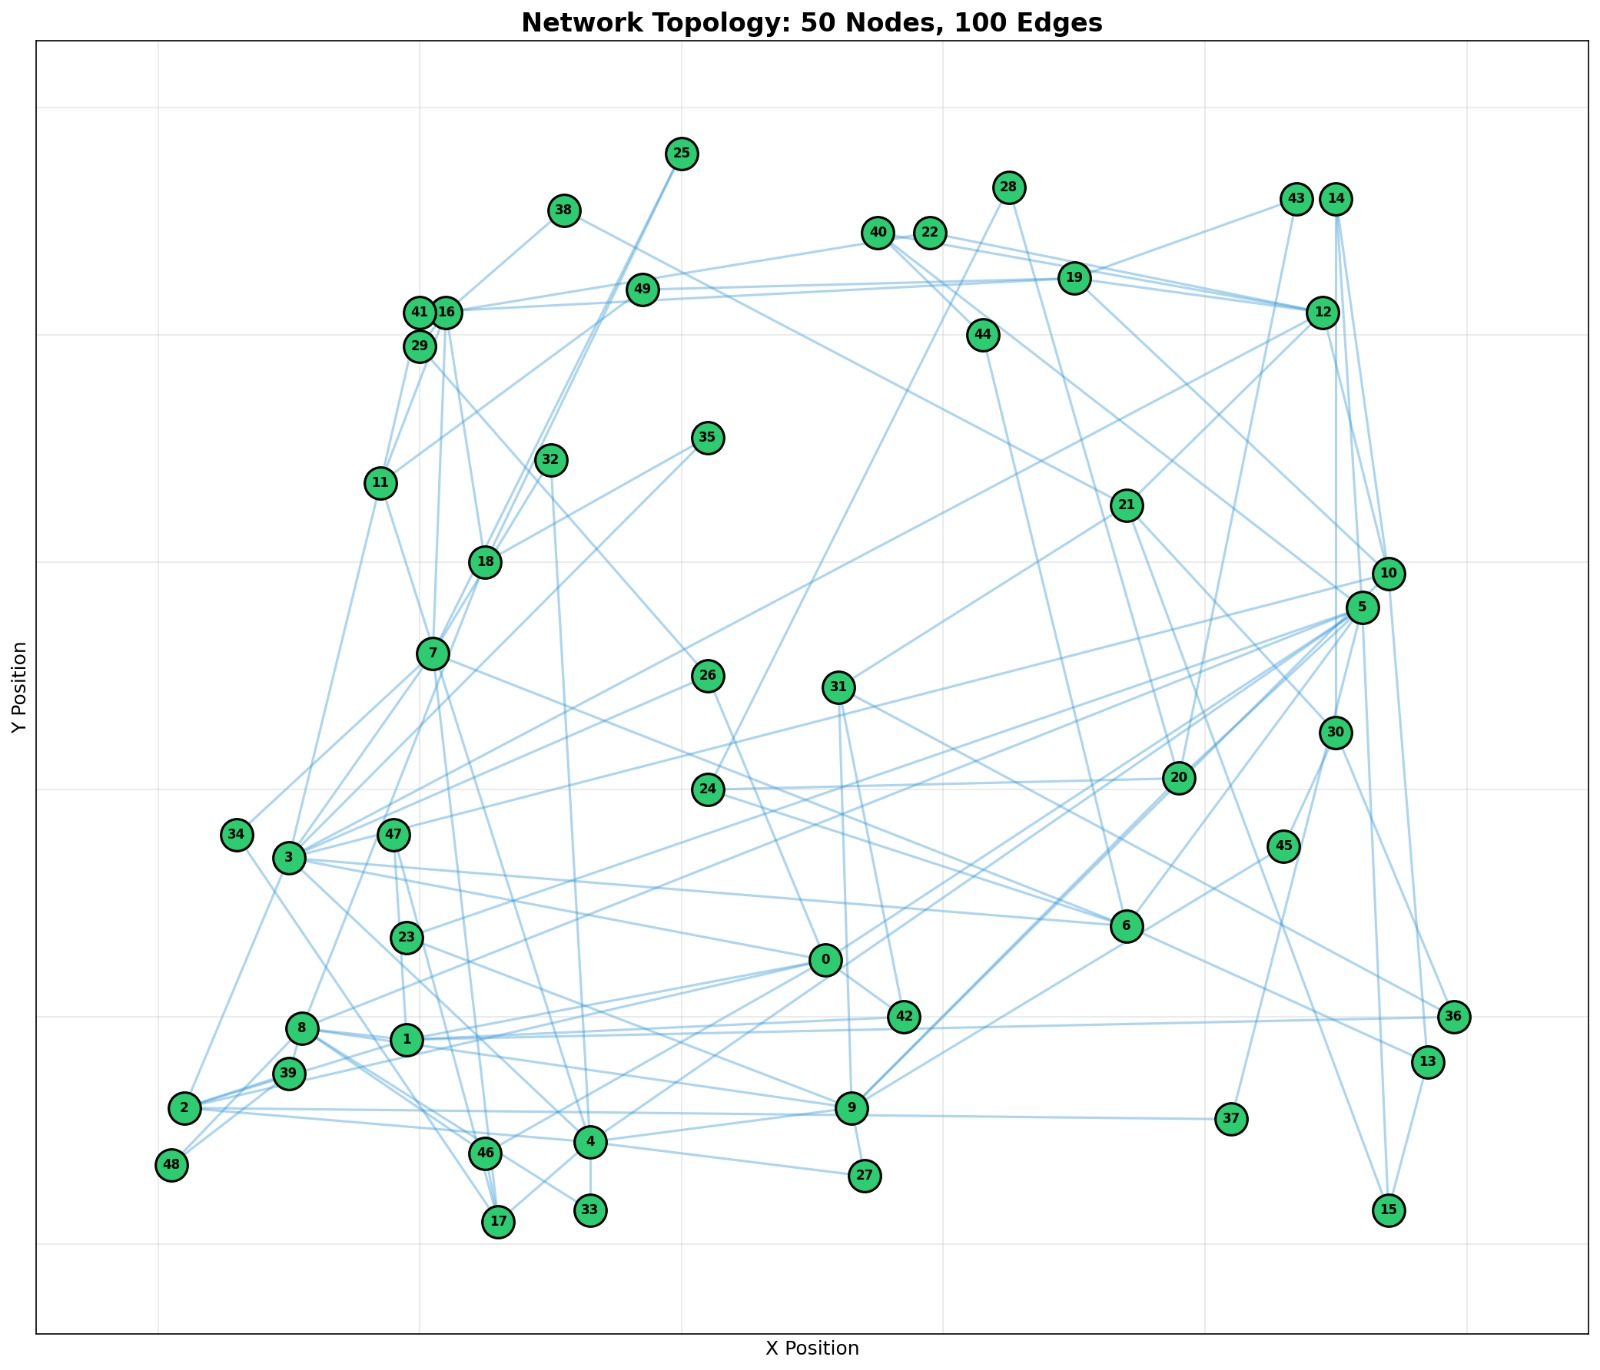
\includegraphics[width=\linewidth]{network.jpeg}
  \caption{Simulated WMN topology: 50 nodes and 100 edges used as the experimental testbed.}
  \label{fig:topology}
\end{figure}

\subsection{Performance Analysis}
The results reveal that the Multi-Agent GAT+DT model consistently outperformed the GAT Baseline across all 3,000 episodes. Despite operating under interference, it converged more rapidly and demonstrated a noticeably stronger ability to identify optimal paths. Table~\ref{tab:performance} summarises the performance metrics for both models.

\begin{table}[htbp]
  \centering
  \caption{Comparative Performance Metrics (3,000 Episodes)}
  \label{tab:performance}
  \begin{tabular}{|l|c|c|}
    \hline
    \textbf{Metric} & \textbf{MA GAT+DT} & \textbf{GAT Baseline} \\
    \hline
    Average Reward           & $+0.93$  & $-17.78$ \\
    \hline
    Avg.\ Path Length (hops) & $3.67$   & $50.85$  \\
    \hline
    Success Rate (\%)        & $96\%$   & $93\%$   \\
    \hline
    Avg.\ Jammed Steps       & $0.29$   & $1.25$   \\
    \hline
    Training Time (min)      & $35.51$  & $75.21$  \\
    \hline
  \end{tabular}
\end{table}

\subsection{Reward and Routing Stability}
The fact that the MA GAT+DT was able to achieve an average reward of $+0.93$, as opposed to $-17.78$, shows that it was able to perform far better than the baseline by a large margin. This is a clear indicator of how effective the Digital Twin model was in reducing interference, path length, and cost due to failed transmissions. The MA GAT+DT, with the combined intelligence of 50 agents, was able to evade areas with high penalty costs, which was not possible for the baseline due to its lack of awareness regarding network changes. The fact that the baseline, with its poor understanding of network dynamics, relied heavily on suboptimal paths meant that it was highly exposed to the cost associated with failed transmissions, hence the low reward achieved.

\begin{figure}[htbp]
  \centering
  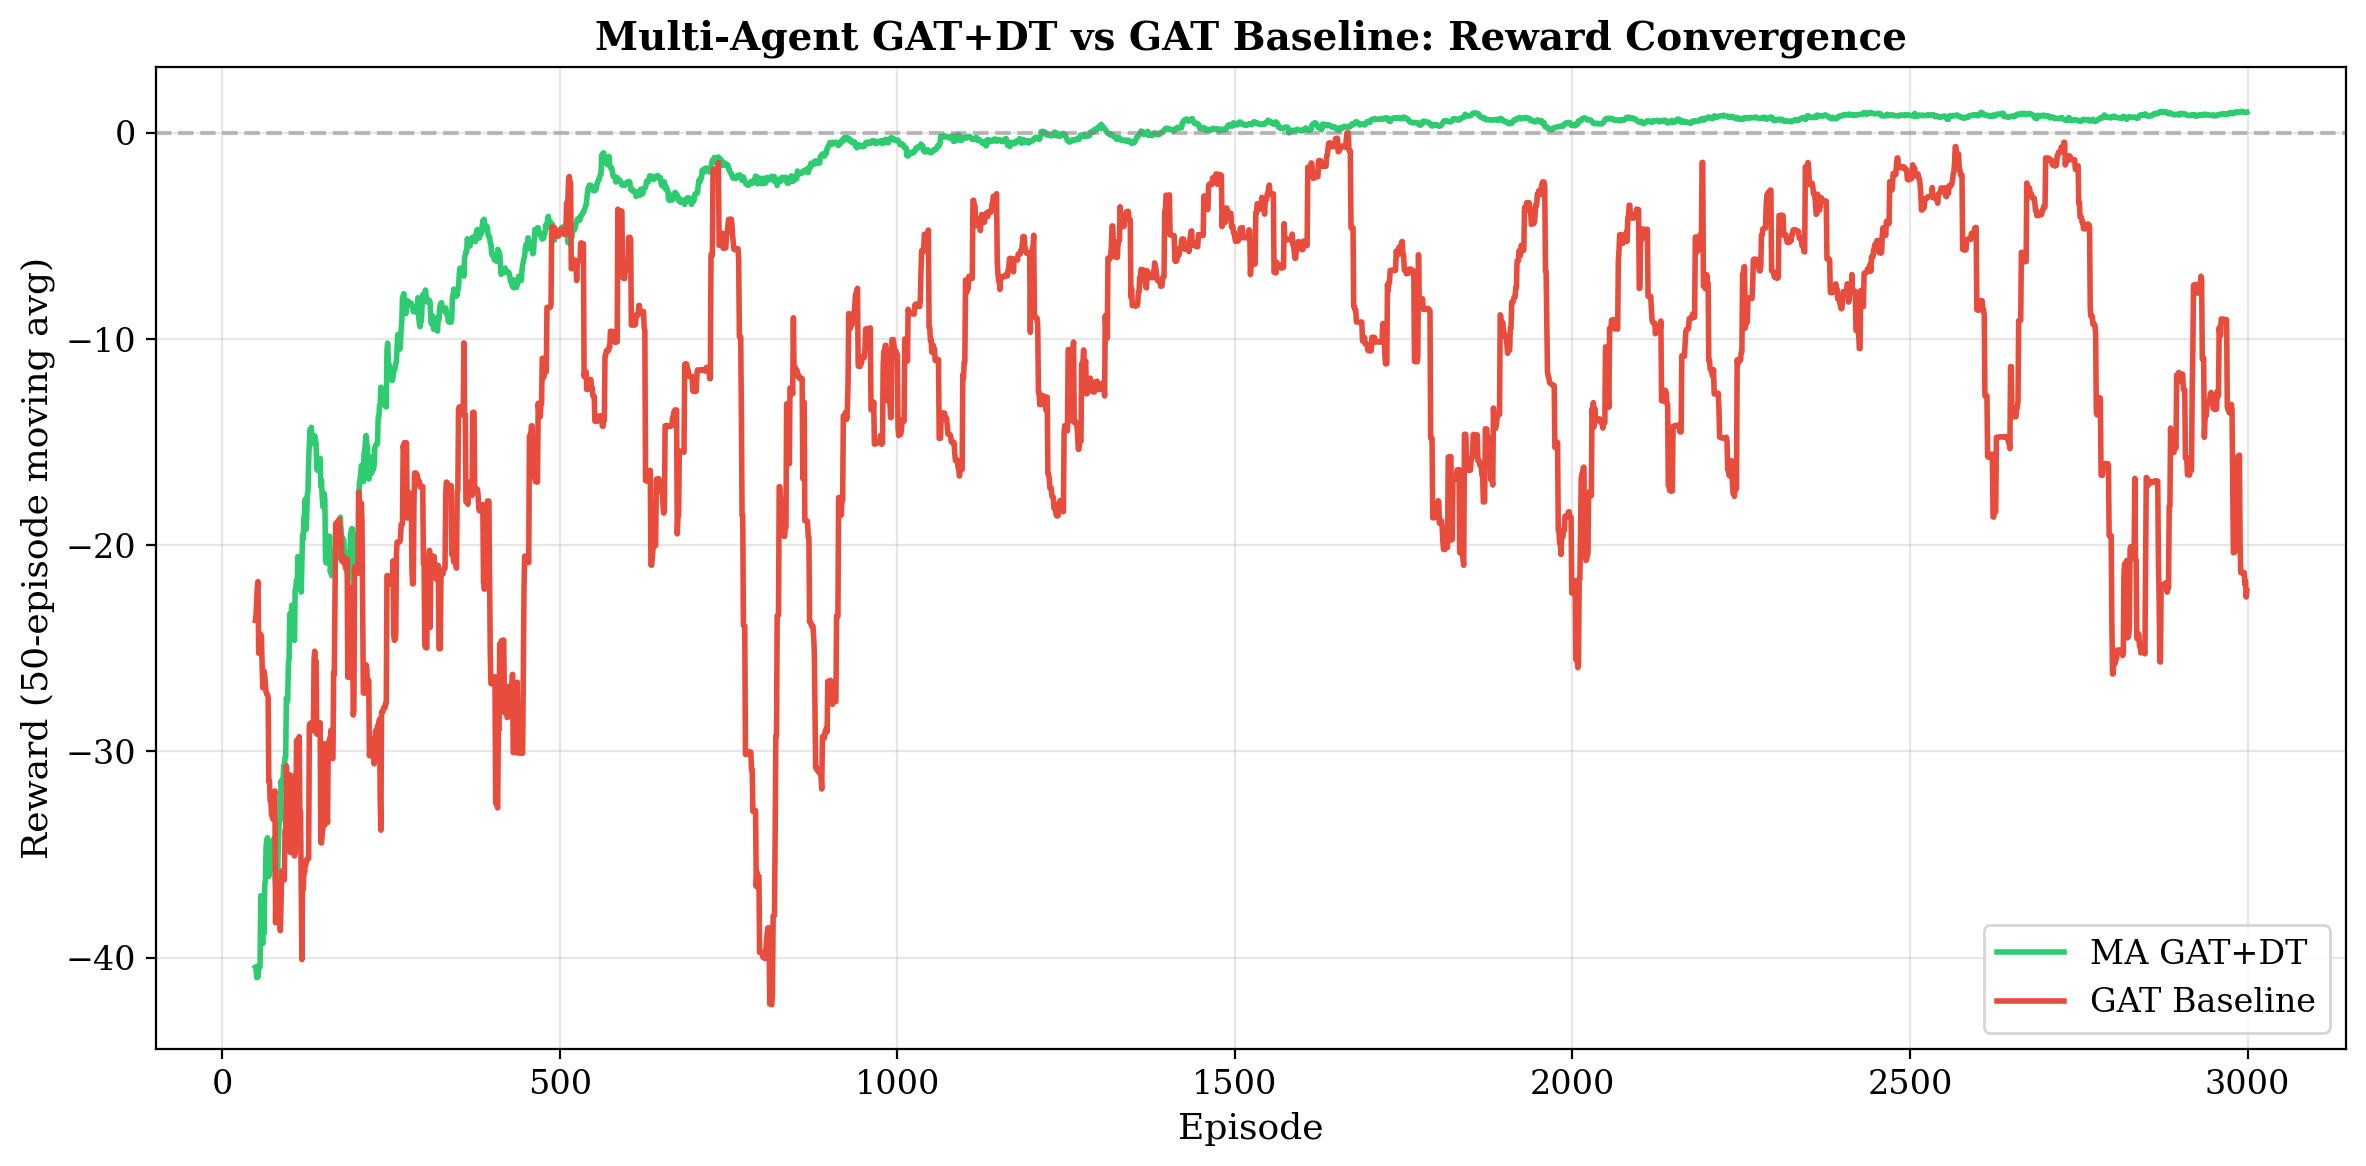
\includegraphics[width=\linewidth]{comparison_reward_graph.png}
  \caption{Reward convergence over 3,000 episodes: MA GAT+DT (Blue) vs.\ GAT Baseline (Orange), 50-episode moving average.}
  \label{fig:reward}
\end{figure}

\subsection{Path Efficiency and End-to-End Latency}
The MA GAT+DT recorded an average path length of $3.67$ hops, which is significantly lower compared to the $50.85$ hops recorded by the GAT Baseline. This proves that the cooperative agents, using features such as jamming probability and node load, which are derived from Digital Twin technology, were consistently able to identify the shortest available paths. This results in fewer relay nodes in each and every route, thereby reducing queuing time and the probability of packet loss. This directly results in a reduction in end-to-end latency.

The GAT Baseline, on the other hand, was unable to identify the shortest available routes and instead consistently chose longer routes. This, in turn, directly resulted in an increase in end-to-end transmission time. The 50 cooperative agents in the MA GAT+DT framework were able to successfully forward the traffic across the network in a much more efficient manner and avoid the problem of nodes being overloaded during this process.

\begin{figure}[htbp]
  \centering
  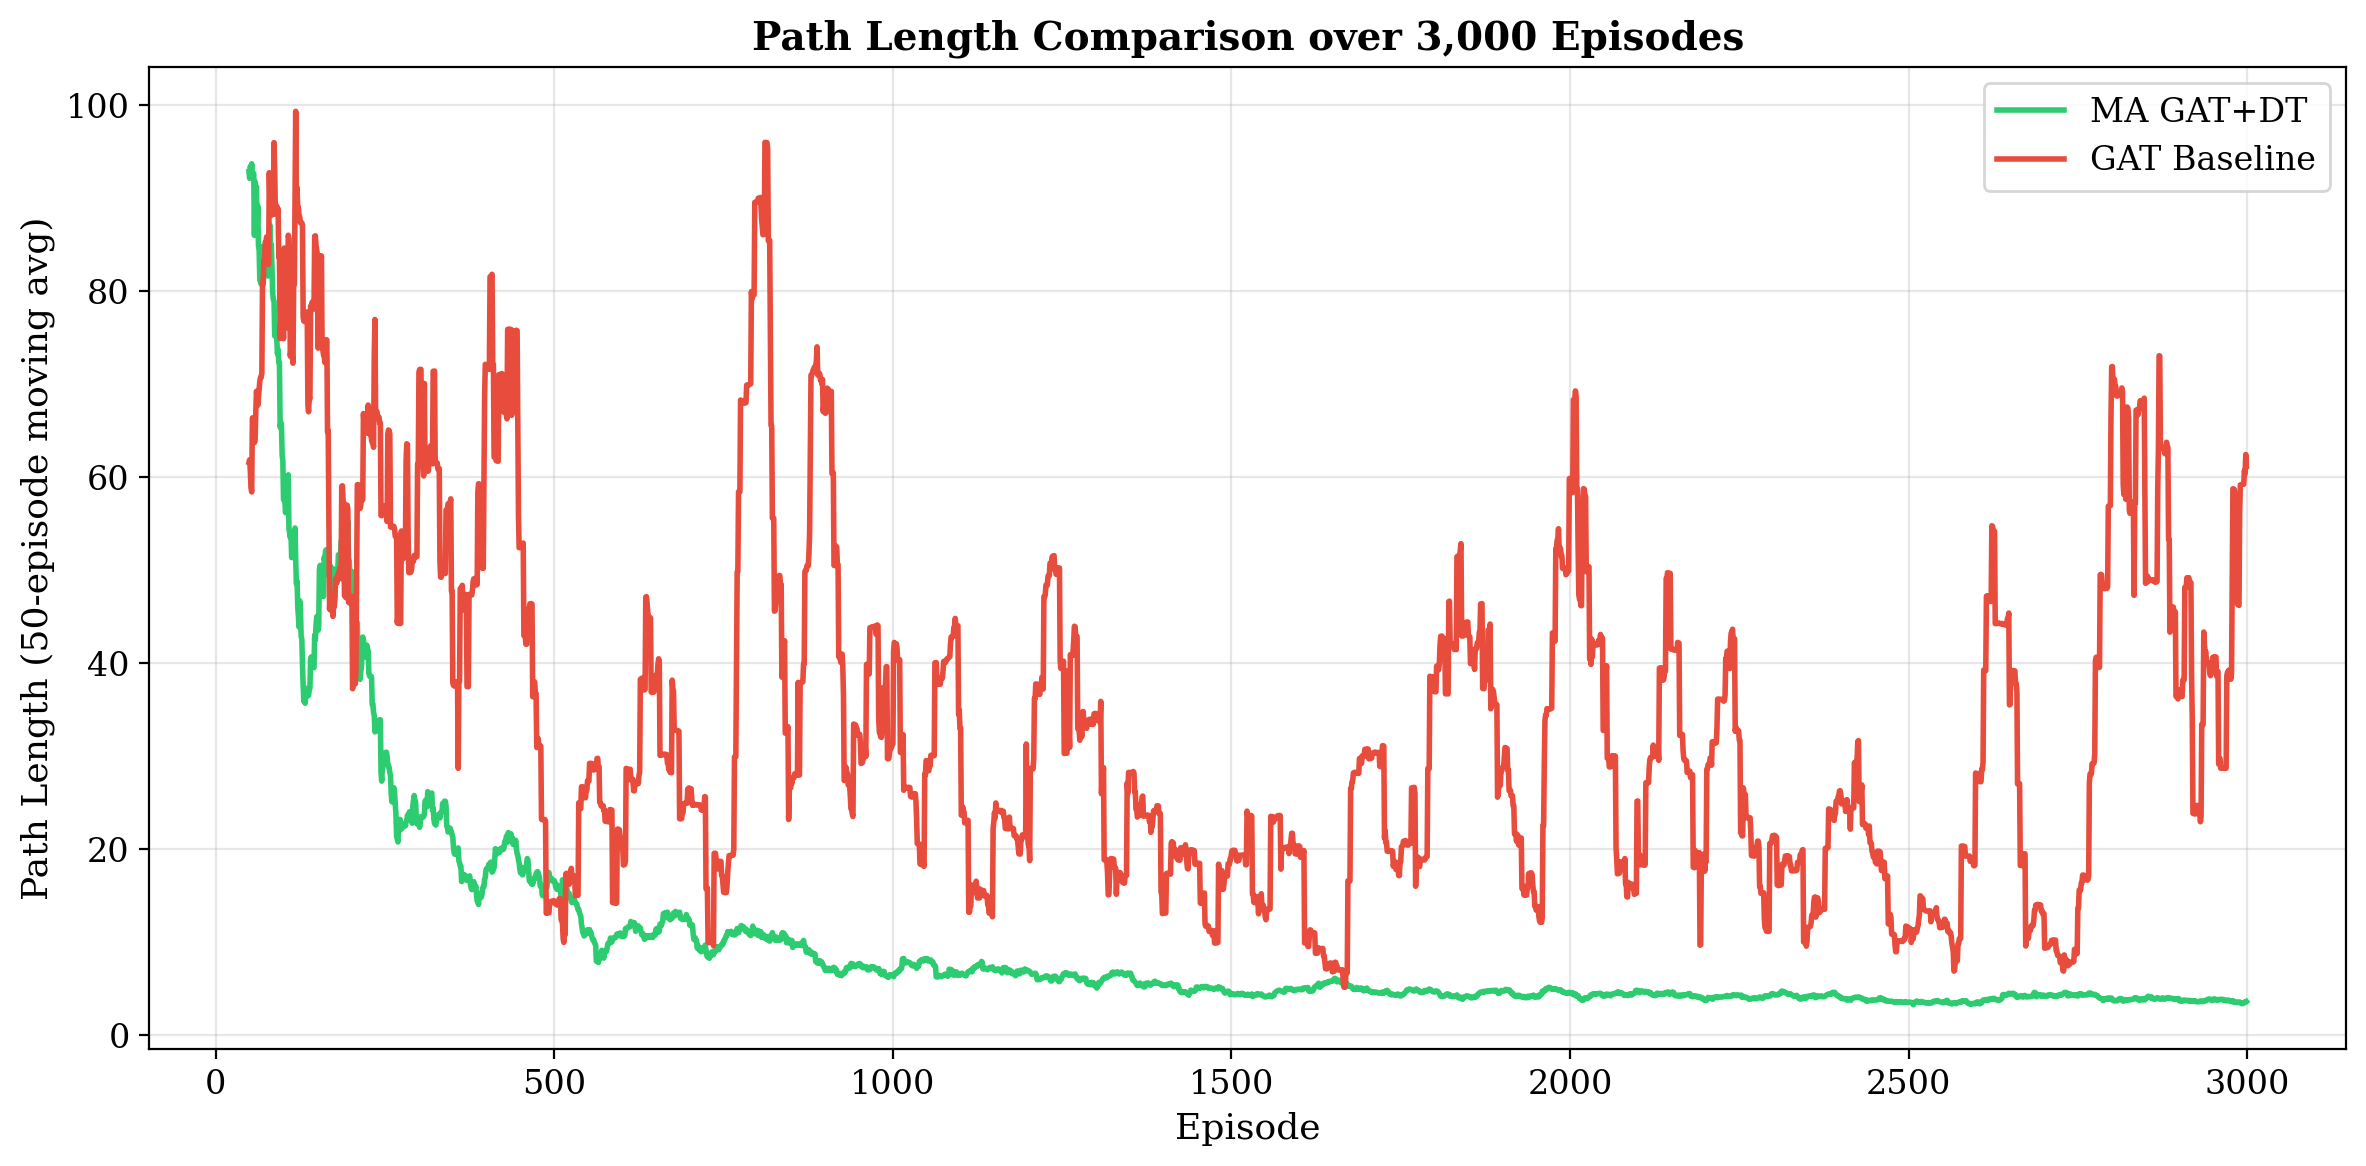
\includegraphics[width=\linewidth]{comparison_path_length_graph.png}
  \caption{Path length comparison over 3,000 episodes: MA GAT+DT converges to near-optimal paths ($\sim$3.67 hops) while the GAT Baseline shows persistently long routes ($\sim$50.85 hops).}
  \label{fig:path_length}
\end{figure}

\subsection{Jamming Avoidance and Network Robustness}
The Average Jammed Steps metric directly measures how well the jamming probability factor performs in cooperative routing. The MA GAT+DT was able to significantly reduce the average jammed steps from $1.25$ to $0.29$, a $76.8\%$ reduction.

This is a clear indication of how the model is able to avoid interference zones and nodes by constantly observing its environment through Digital Twin. It is therefore guaranteed that link reliability and communication stability will always be preserved, even in complex situations. The fact that this is done concurrently for 50 agents, and the results are distributed among all active routing paths, is a guarantee of this conclusion.

\begin{figure}[htbp]
  \centering
  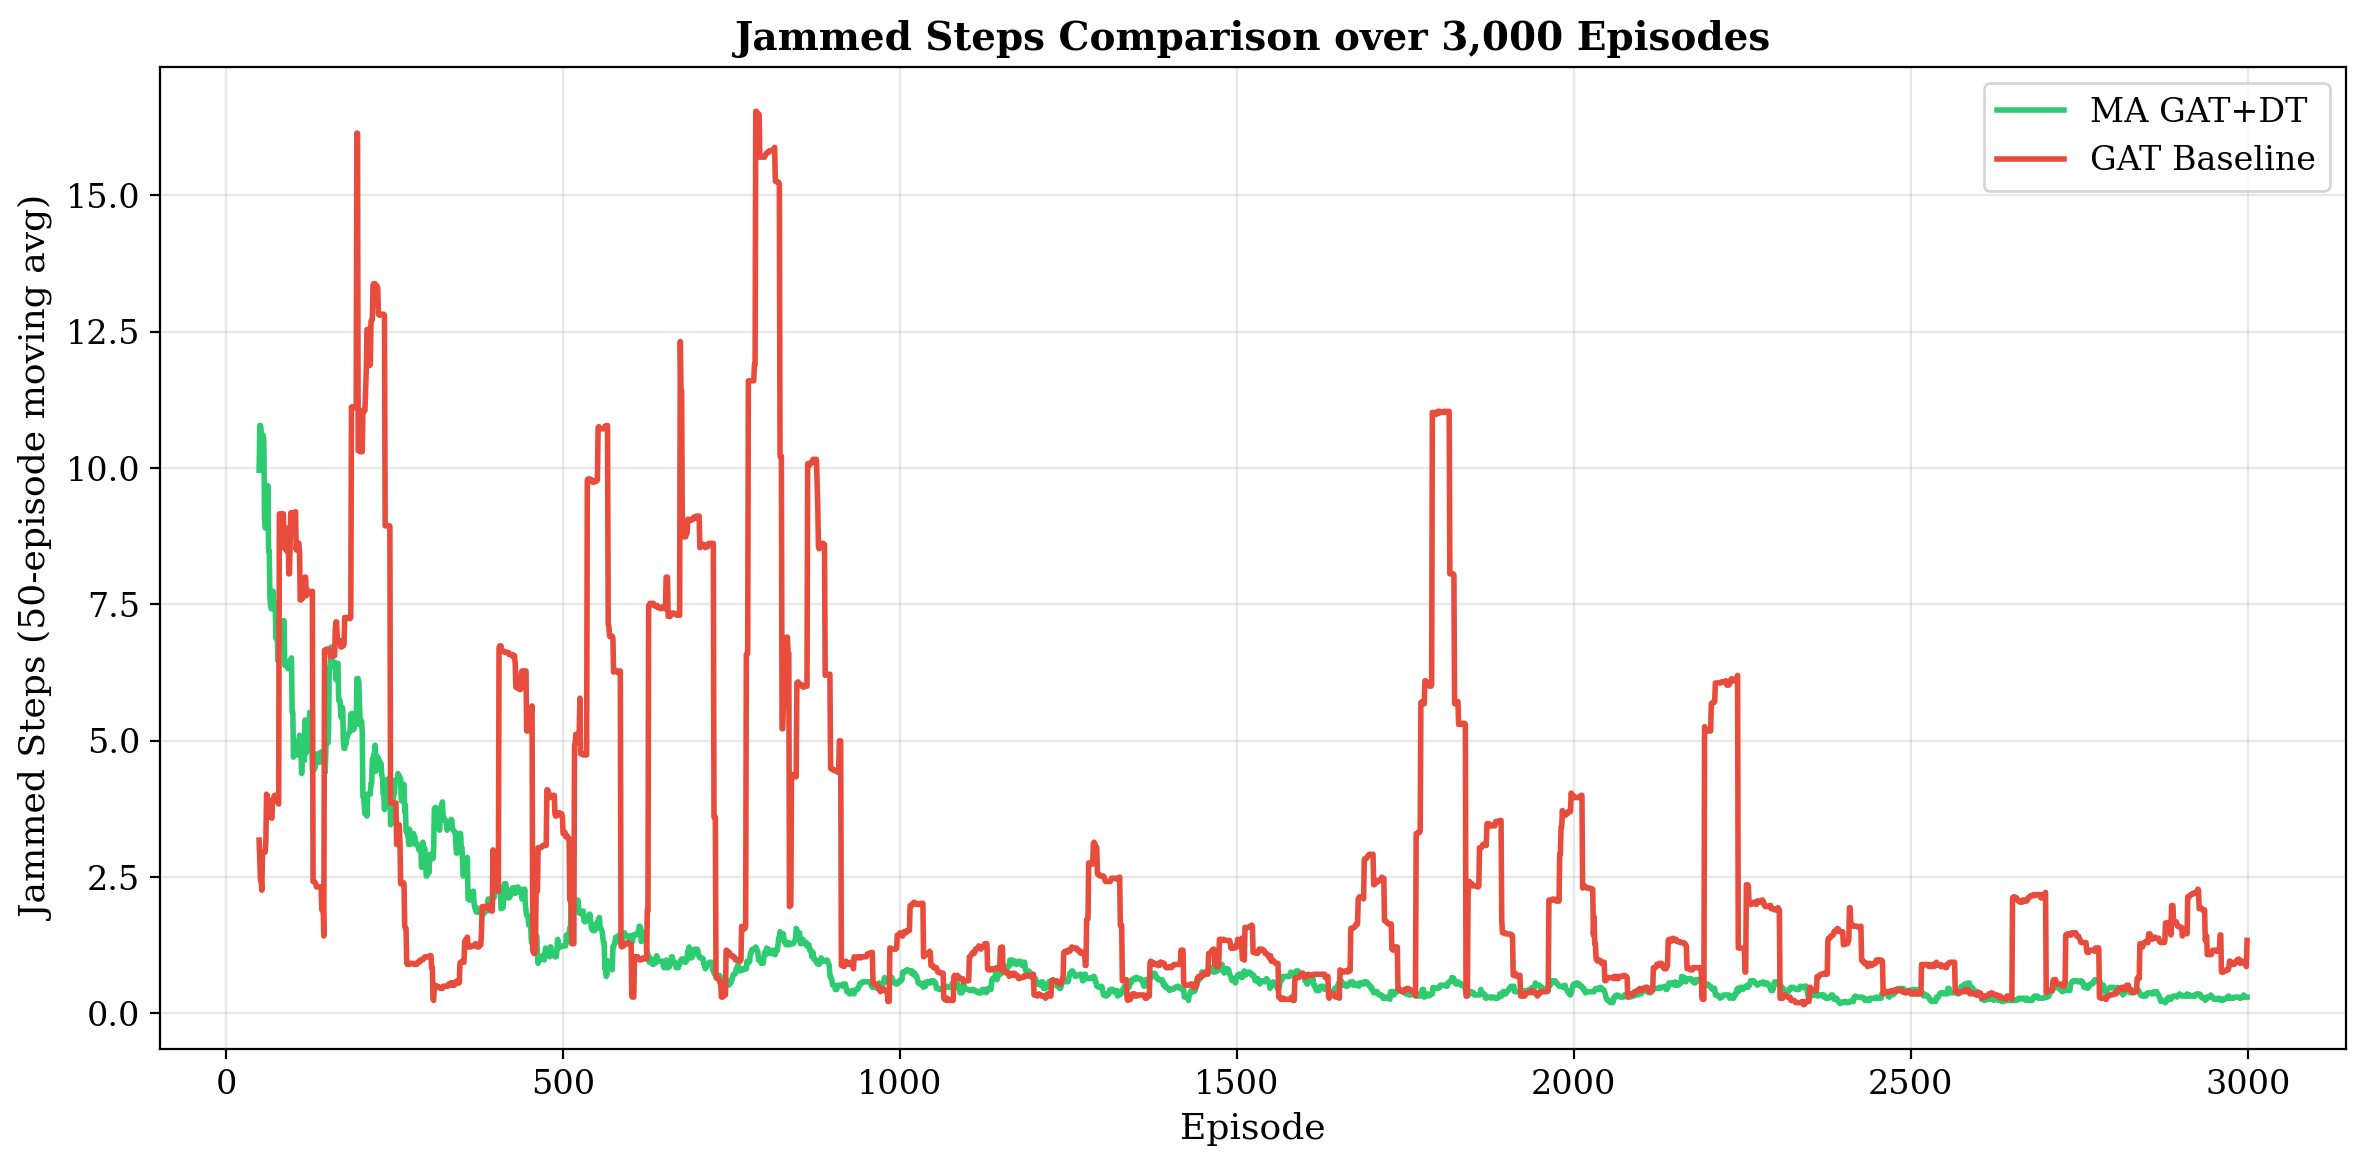
\includegraphics[width=\linewidth]{comparison_jammed_steps_graph.png}
  \caption{Jammed steps comparison over 3,000 episodes: MA GAT+DT maintains near-zero jammed steps while the GAT Baseline shows persistent interference exposure.}
  \label{fig:jammed}
\end{figure}

\subsection{Convergence Behaviour and Training Efficiency}
The MA GAT+DT completed 3,000 training episodes in $35.51$ minutes, compared to $75.21$ minutes for the GAT Baseline, reaching a speed advantage of $52.8\%$ while coordinating 50 agents, each with their own policy network. This quicker convergence is primarily due to the shared experience replay mechanism, which allows cooperative agents to more effectively explore the state space, speeding policy learning.

In terms of packet delivery, the MA GAT+DT obtained a success rate of $96\%$ compared to the baseline of $93\%$. The quality of effective routing was also significantly higher, with an average reward of $+0.93$ vs $-17.78$, and an average path length of $3.67$ hops versus $50.85$. These findings demonstrate that the MA GAT+DT regularly beats the baseline in all examined performance indicators.

\begin{figure}[htbp]
  \centering
  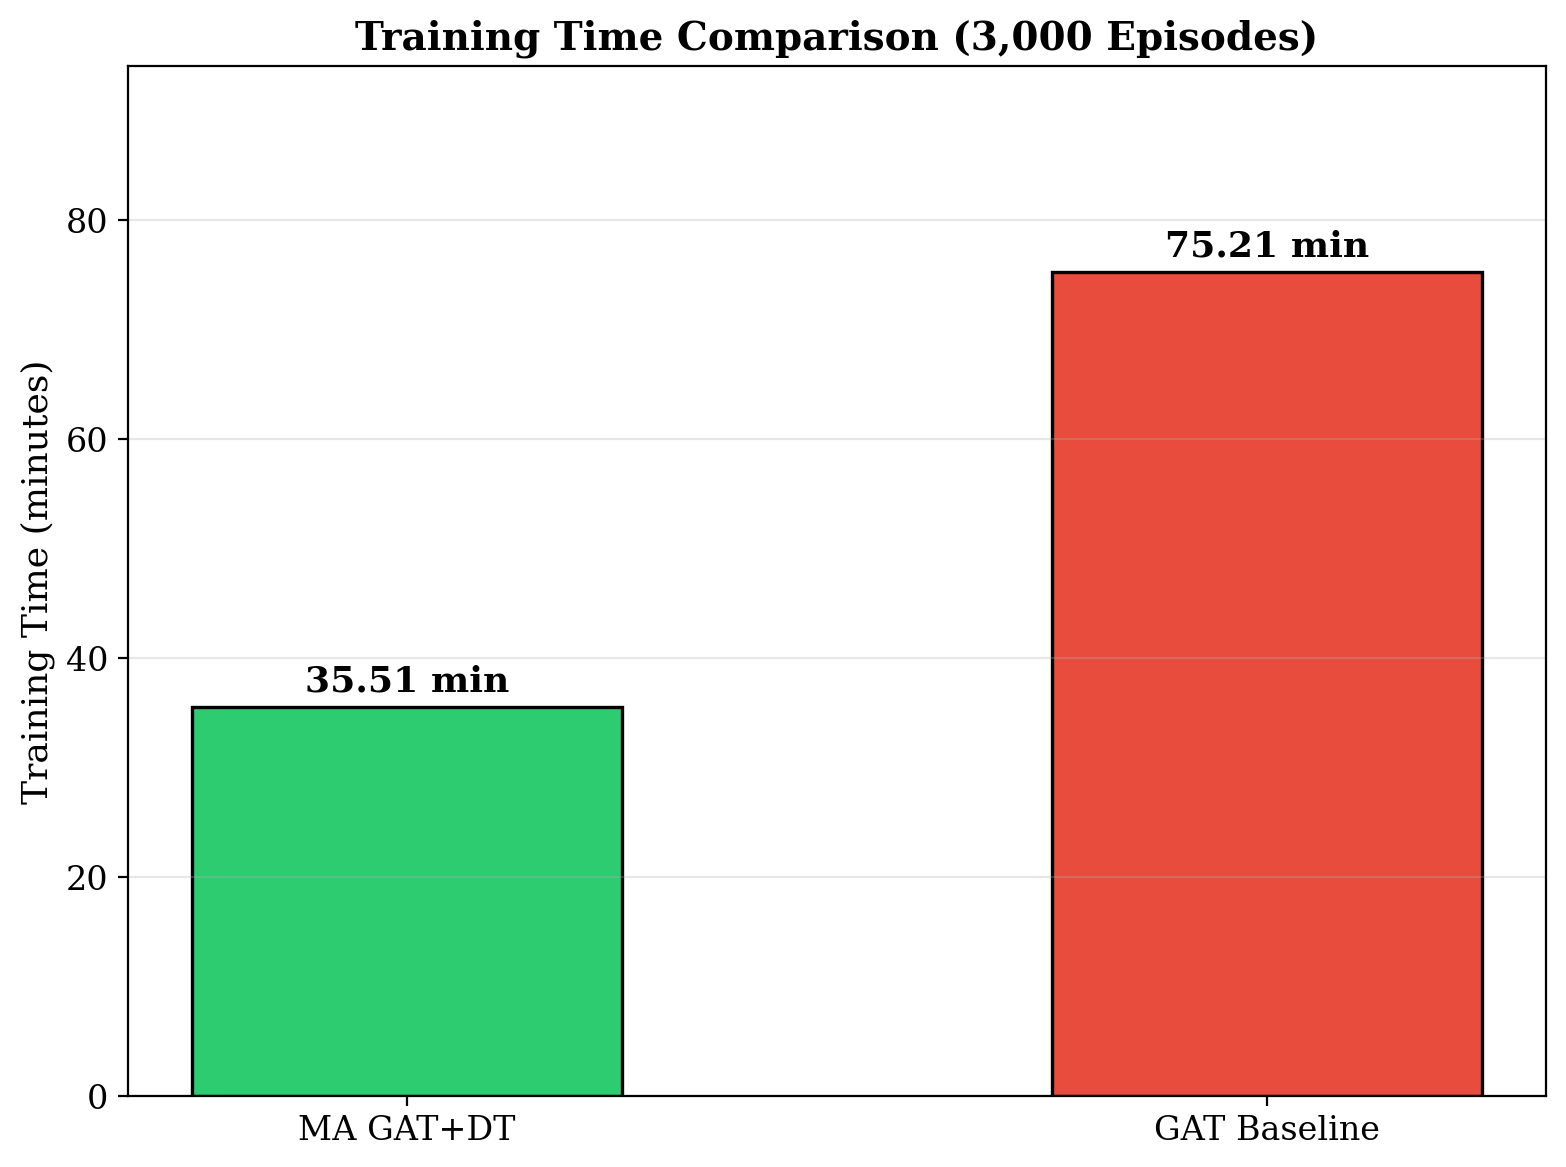
\includegraphics[width=0.85\linewidth]{comparison_time_graph.png}
  \caption{Training time comparison for 3,000 episodes: MA GAT+DT (35.51 min) vs.\ GAT Baseline (75.21 min).}
  \label{fig:training_time}
\end{figure}

\subsection{Success Rate and Reliability}
The MA GAT+DT attained a success rate of $96\%$ against the GAT Baseline's $93\%$, establishing a clear edge in reliable packet delivery. But the real difference lies in routing quality. The MA GAT+DT delivers a substantially higher average reward of $+0.93$ compared to $-17.78$, produces routes nearly 14 times shorter, and encounters considerably less interference. The baseline's longer routes make it both less efficient and far more vulnerable to interference, collectively dragging down its success rate and route quality.

Backed by its cooperative multi-agent architecture and continuous Digital Twin awareness, the MA GAT+DT has already developed high-quality routing policies that surpass the baseline across every measured metric. With further training, these advantages are only expected to strengthen.

%------------------------------------------------------------------
\section{Conclusion}
This paper presents an integrated resilience architecture that leverages Digital Twin modeling, Graph Attention Networks, and Multi-Agent Deep Q-Networks to facilitate adaptive and jamming-aware routing in Wireless Mesh Networks. In 3,000 training episodes, the proposed MA GAT+DT model surpassed the performance of the GAT Baseline model and converged $52.8\%$ faster. Further research directions could be explored in the application of transfer learning, in which the pre-trained MA GAT+DT model can generalize across different wireless mesh network topologies without retraining from scratch. Moreover, testing the framework in actual hardware testbeds with live radio interferers can serve as a validation of the Digital Twin's accuracy outside the simulated environment.

\begin{thebibliography}{00}
\bibitem{pappone2023}
A.~Pappone \textit{et al.}, ``Graph Neural Network and Multi-Agent Deep Reinforcement Learning for Adaptive Routing in Wireless Mesh Networks,'' 2023.

\bibitem{jin2025}
Z.~Jin, H.~Xu, Z.~Kong, and C.~Pan, ``A Resilient Routing Strategy Based on Deep Reinforcement Learning for Urban Emergency Communication Networks,'' \textit{IEEE Trans. Veh. Technol.}, 2024/2025 (pre-print).

\bibitem{kipf2017}
T.~N.~Kipf and M.~Welling, ``Semi-Supervised Classification with Graph Convolutional Networks,'' in \textit{Proc. ICLR}, 2017.

\bibitem{velickovic2018}
P.~Veli\v{c}kovi\'{c} \textit{et al.}, ``Graph Attention Networks,'' in \textit{Proc. ICLR}, 2018.

\bibitem{krause2023}
A.~Krause, M.~D.~Khursheed, P.~Schulz, F.~Burmeister, and G.~Fettweis, ``The Digital Twin of the Radio Environment: A Novel Approach for Anomaly Detection,'' \textit{IEEE Commun. Mag.}, 2023.

\bibitem{meenakshi2023}
S.~Meenakshi and R.~Shriram, ``Enhancing Fault Tolerance in WMNs Through Adaptive and Resilient Routing Protocols,'' in \textit{Proc. 2023 Int. Conf. Data Sci., Agents \& Artif. Intell. (ICDSAAI)}, IEEE, 2023.

\bibitem{koutsonikolas2024}
D.~Koutsonikolas \textit{et al.}, ``Asynchronous and Distributed Self-Healing for Mesh Networks,'' \textit{IEEE/ACM Trans. Netw.}, 2024 (pre-print).

\bibitem{rajesh2020}
M.~Rajesh and G.~A.~S.~Kumar, ``A Robust Design of Fault Nodes Identification and Recovery Model over Wireless Sensor Network,'' \textit{Wireless Pers. Commun.}, Springer, 2020.

\bibitem{zhang2023}
Y.~Zhang \textit{et al.}, ``Few-Shot Transfer Learning-Based Fault Classification in Wireless Sensor Networks,'' \textit{IEEE Trans. Instrum. Meas.}, IEEE, 2023.

\bibitem{sun2022}
Y.~Sun, M.~Bennis \textit{et al.}, ``Multi-Agent Reinforcement Learning for Dynamic Topology Optimization of Mesh Wireless Networks,'' \textit{IEEE Trans. Commun.}, IEEE, 2022.



\bibitem{prasad2023}
R.~Prasad and R.~K.~Baghel, ``A Distributed Self-Detection Based Fault Diagnosis for Wireless Sensor Networks,'' \textit{Ad Hoc Netw.}, vol.~149, Elsevier, 2023.



\bibitem{chen2024}
Y.~Chen, X.~Xu, J.~Li, and H.~Wu, ``Adaptive Fault-Tolerant Routing Using Federated Reinforcement Learning in Wireless Mesh Networks,'' \textit{IEEE Internet Things J.}, vol.~11, no.~4, pp.~5123--5137, Apr. 2024.

\bibitem{lanka2023}
V.~Lanka, ``Multi-Agent Reinforcement Learning (MARL),'' \textit{Medium}, 2023. [Online]. Available: \url{https://vinaylanka.medium.com/multi-agent-reinforcement-learning-marl-1d55dfff6439}

\bibitem{ahu_resilient_routing}
``Resilient-Routing-in-Wireless-Mesh-Networks-using-Digital-Twin-and-GNN-Based-Reinforcement-Learning,'' \textit{GitHub repository}, 2026 Available:\url{https://github.com/anandahu/Resilient-Routing-in-Wireless-Mesh-Networks-using-Digital-Twin-and-GNN-Based-Reinforcement-Learning}

\bibitem{ahu_gat_dataset}
GAT-MADT\_dataset,'' \textit{GitHub repository}, 2026.Available: \url{https://github.com/anandahu/GAT-MADT_dataset}

\bibitem{krause_dt_radio_dataset}

\textit{Dataset}, Zenodo, Jan. 2024.
[Online]. Available: \url{https://doi.org/10.5281/zenodo.10512316}

\end{thebibliography}

\end{document}
```